\newcommand{\grasp}{\lr{GRASP}}
\newcommand{\controller}{\lr{Controller Pattern}}
\newcommand{\expert}{\lr{Expert Pattern}}

\chapter{اعمال الگو‌های واگذاری مسئولیت}
\section{توضیح الگو‌های استفاده شده}
توضیحات این بخش در جداول 
\ref{table-with-pic:1}،
\ref{table-with-pic:2}،
\ref{table-with-pic:3}،
\ref{table-with-pic:4}،
\ref{table-with-pic:5}،
\ref{table-with-pic:6} و 
\ref{table-with-pic:7}
آورده شده‌اند.

\begin{table}[H]
\begin{adjustbox}{width=\textwidth}
\begin{tabular}{|c|p{\textwidth}|}
\hline
نام &
کنترل‌گر ثبت آگهی \\ 
\hline
گونه & 
\grasp \\
\hline
خانواده &
\controller \\
\hline
مسئله & 
چه کسی مسئول رسیدگی به درخواست ثبت آگهی است؟\\
\hline
راه‌حل& 
اطلاعات بانکی و داده‌ها را از کاربر گرفته به کنترل‌گر ثبت آگهی داده می‌شود. \\
\hline
ساختاری & 
\begin{minipage}{\textwidth}
	\begin{flushleft}
		\begin{minipage}{\textwidth}
			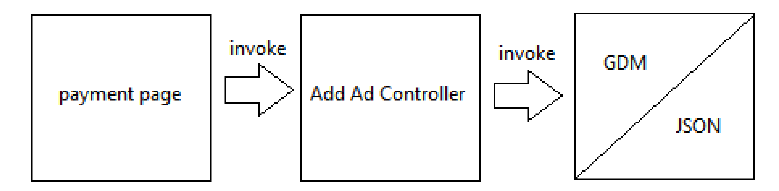
\includegraphics[width=13cm, height=2.7cm]{./images/7-1-1}
		\end{minipage}
	\end{flushleft}
\end{minipage}
	
\\
\hline
رفتاری & 
\begin{minipage}{\textwidth}
	\begin{flushleft}
		\begin{minipage}{\textwidth}
			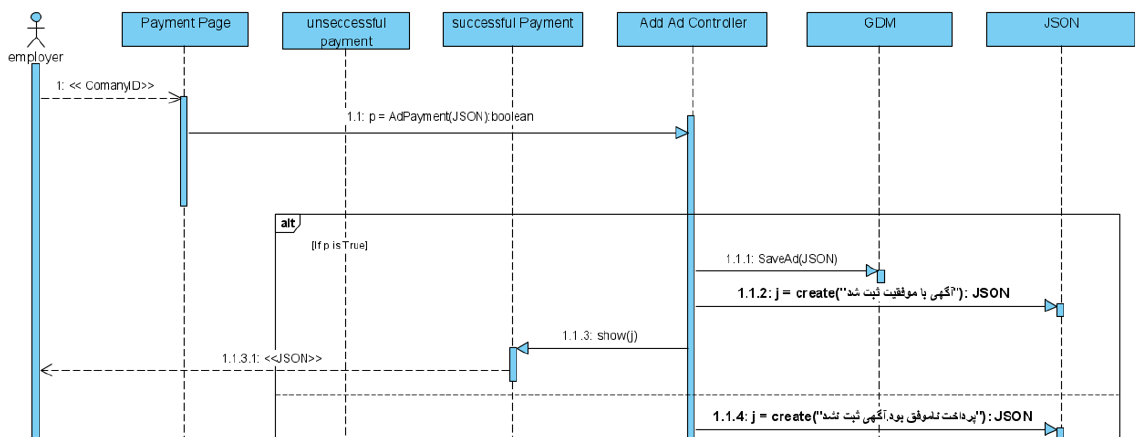
\includegraphics[width=13.5cm, height=6cm]{./images/7-1-2}
		\end{minipage}
	\end{flushleft}
\end{minipage}
\\
\hline
\end{tabular}
\end{adjustbox}
\caption{جدول \arabic{table}}
\label{table-with-pic:1}
\end{table}

\begin{table}[H]
	\begin{adjustbox}{width=\textwidth}
		\begin{tabular}{|c|p{\textwidth}|}
			\hline
			نام &
			کنترل‌گر جستجوی آگهی \\ 
			\hline
			گونه & 
			\grasp \\
			\hline
			خانواده &
			\controller \\
			\hline
			مسئله & 
			چه کسی مسئول رسیدگی به جستجوی آگهی است؟\\
			\hline
			راه‌حل& 
نوار جستجو در صفحه‌ی اصلی، عبارت جستجو را به کنترل‌گر جستجوی آگهی داده و در نهایت نتیجه را به صفحه‌ی نتایج جستجو ارسال می‌کند. \\
			\hline
			ساختاری & 
			\begin{minipage}{\textwidth}
				\begin{flushleft}
					\begin{minipage}{\textwidth}
						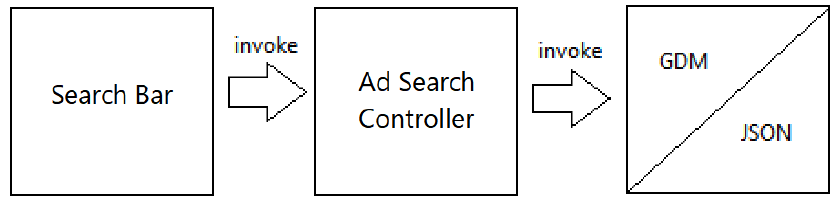
\includegraphics[width=13cm, height=2.7cm]{./images/7-2-1}
					\end{minipage}
				\end{flushleft}
			\end{minipage}
			
			\\
			\hline
			رفتاری & 
			\begin{minipage}{\textwidth}
				\begin{flushleft}
					\begin{minipage}{\textwidth}
						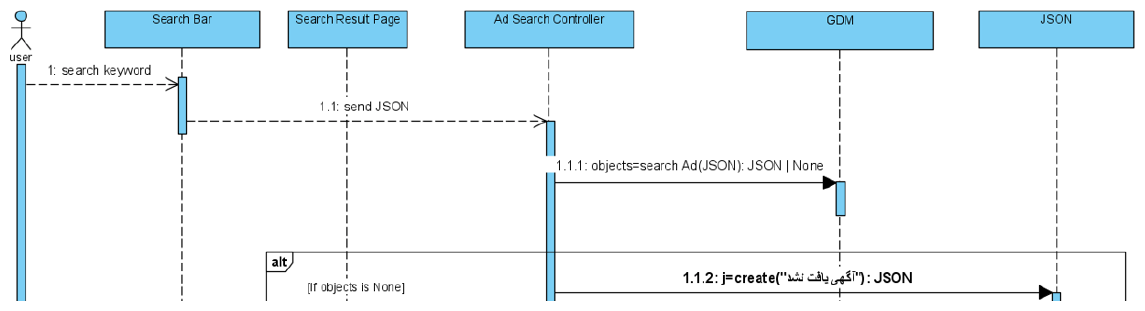
\includegraphics[width=13.5cm, height=6cm]{./images/7-2-2}
					\end{minipage}
				\end{flushleft}
			\end{minipage}
			\\
			\hline
		\end{tabular}
	\end{adjustbox}
	\caption{جدول \arabic{table}}
	\label{table-with-pic:2}
\end{table}

\begin{table}[H]
	\begin{adjustbox}{width=\textwidth}
		\begin{tabular}{|c|p{\textwidth}|}
			\hline
			نام &
			کنترل‌گر مشاهده‌ی رزومه \\ 
			\hline
			گونه & 
			\grasp \\
			\hline
			خانواده &
			\controller \\
			\hline
			مسئله & 
			چه کسی مسئول روند نمایش رزومه است؟\\
			\hline
			راه‌حل& 
			درخواست و اطلاعات مربوطه را به کنترل‌گر مشاهده‌ی رزومه فرستاده و کنترل‌گر نتبجه را به صفحه‌ی نمایش رزومه ارسال می‌کند. \\
			\hline
			ساختاری & 
			\begin{minipage}{\textwidth}
				\begin{flushleft}
					\begin{minipage}{\textwidth}
						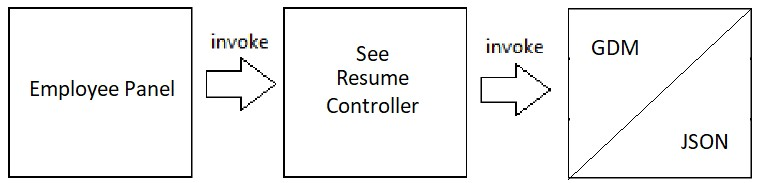
\includegraphics[width=13cm, height=2.7cm]{./images/7-3-1}
					\end{minipage}
				\end{flushleft}
			\end{minipage}
		
			\\
			\hline
			رفتاری & 
			\begin{minipage}{\textwidth}
				\begin{flushleft}
					\begin{minipage}{\textwidth}
						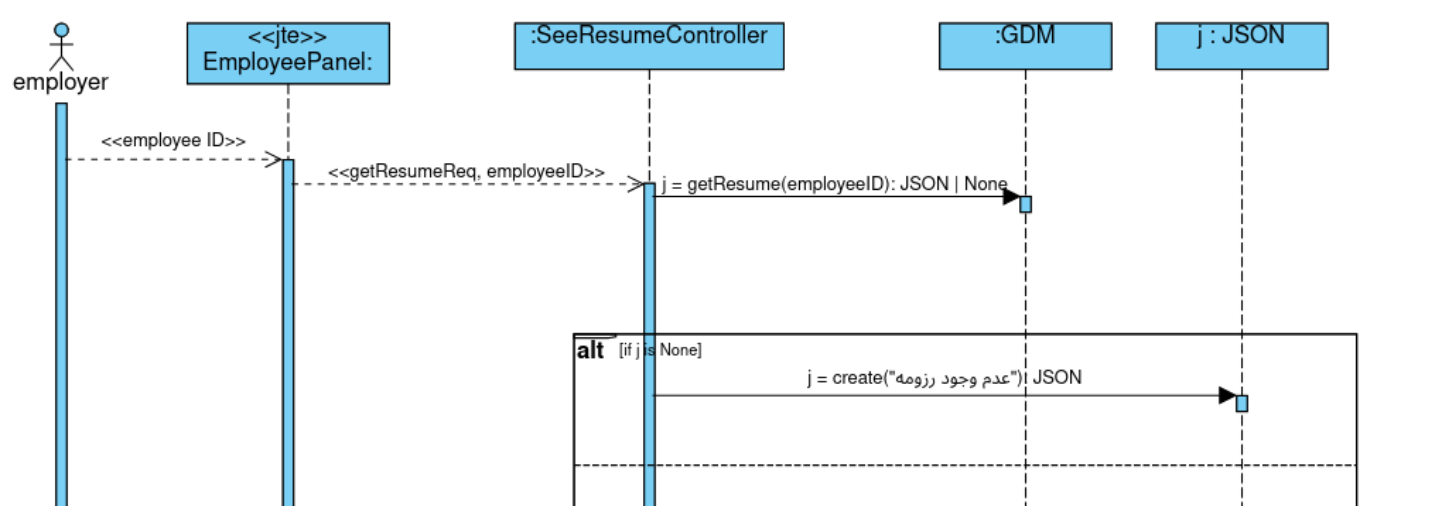
\includegraphics[width=13.5cm, height=6cm]{./images/7-3-2}
					\end{minipage}
				\end{flushleft}
			\end{minipage}
			\\
			\hline
		\end{tabular}
	\end{adjustbox}
	\caption{جدول \arabic{table}}
	\label{table-with-pic:3}
\end{table}

\begin{table}[H]
	\begin{adjustbox}{width=\textwidth}
		\begin{tabular}{|c|p{\textwidth}|}
			\hline
			نام &
			کنترل‌گر نشان‌دار کردن آگهی \\ 
			\hline
			گونه & 
			\grasp \\
			\hline
			خانواده &
			\lr{Expert Pattern} \\
			\hline
			مسئله & 
			چه کسی مسئول نشان‌دار کردن آگهی است؟\\
			\hline
			راه‌حل& 
			صفحه‌ی آگهی، اطلاعات مربوط به آگهی، کارجو و درخواستی مبنی بر نشان‌دار کردن آگهی را به کنترل‌گر نشان‌دار کردن آگهی ارسال می‌کند و کنترل‌گر نتیجه را به صفحه‌ی آگهی ارسال می‌کند. \\
			\hline
			ساختاری & 
			\begin{minipage}{\textwidth}
				\begin{flushleft}
					\begin{minipage}{\textwidth}
						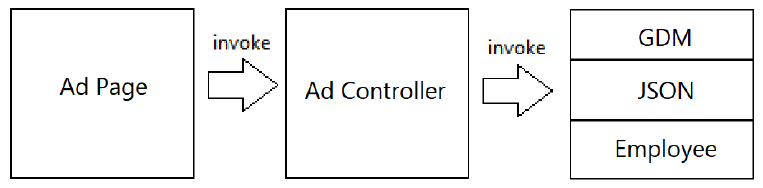
\includegraphics[width=13cm, height=2.7cm]{./images/7-4-1}
					\end{minipage}
				\end{flushleft}
			\end{minipage}
			
			\\
			\hline
			رفتاری & 
			\begin{minipage}{\textwidth}
				\begin{flushleft}
					\begin{minipage}{\textwidth}
						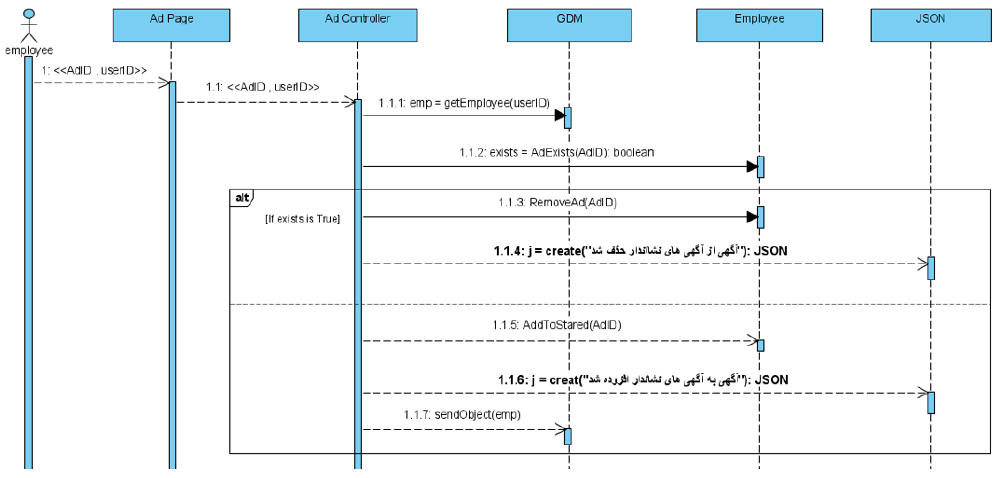
\includegraphics[width=13.5cm, height=6cm]{./images/7-4-2}
					\end{minipage}
				\end{flushleft}
			\end{minipage}
			\\
			\hline
			الگو‌های مرتبط & 
			با توجه به اینکه در این نمودار از \lr{usecase controller} باعث بوجود آمدن تورم می‌شود، از الگوی خبره برای نشان‌دار کردن آگهی استفاده شده است. \\
			\hline
		\end{tabular}
	\end{adjustbox}
	\caption{جدول \arabic{table}}
	\label{table-with-pic:4}
\end{table}

\begin{table}[H]
	\begin{adjustbox}{width=\textwidth}
		\begin{tabular}{|c|p{\textwidth}|}
			\hline
			نام &
			کنترل‌گر آگهی‌های درخواستی \\ 
			\hline
			گونه & 
			\grasp \\
			\hline
			خانواده &
			\controller \\
			\hline
			مسئله & 
			چه کسی مسئول نمایش روند آگهی‌های درخواستی کارجو است؟\\
			\hline
			راه‌حل& 
			صفحه‌ی پنل ‌کاربری، درخواستی مبنی بر دریافت آگهی‌های درخواستی به کنترل‌گر آگهی‌های درخواستی می‌فرستد و نتیجه را از کنترل‌گر آگهی به پنل کاربری ارسال می‌کند. \\
			\hline
			ساختاری & 
			\begin{minipage}{\textwidth}
				\begin{flushleft}
					\begin{minipage}{\textwidth}
						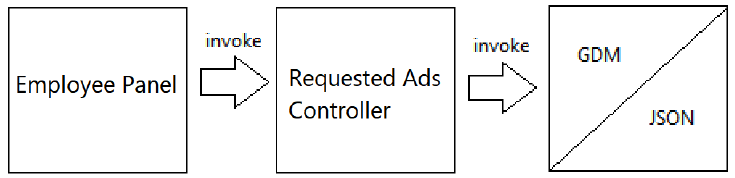
\includegraphics[width=13cm, height=2.7cm]{./images/7-5-1}
					\end{minipage}
				\end{flushleft}
			\end{minipage}
			
			\\
			\hline
			رفتاری & 
			\begin{minipage}{\textwidth}
				\begin{flushleft}
					\begin{minipage}{\textwidth}
						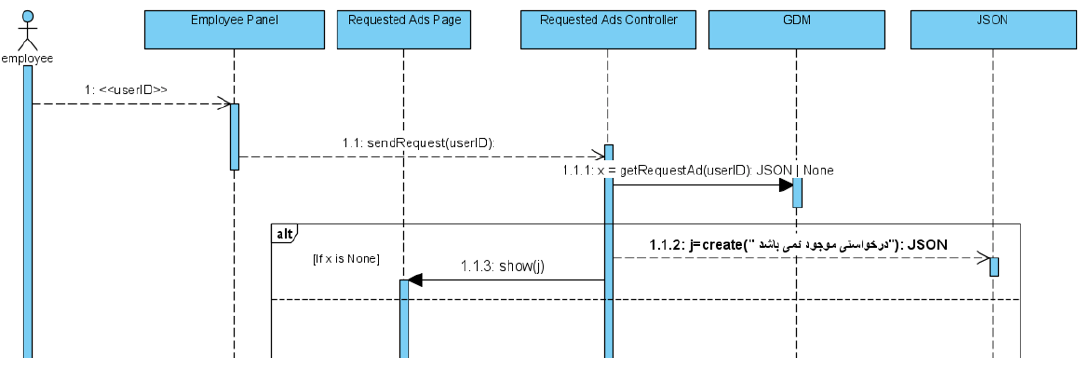
\includegraphics[width=13.5cm, height=6cm]{./images/7-5-2}
					\end{minipage}
				\end{flushleft}
			\end{minipage}
			\\
			\hline
						الگو‌های مرتبط &
						این الگو در سیستم‌های تعاملی پیاده‌سازی اشیاء آن مورد استفاده قرار می‌گیرد. در این نمودار مورد کاربرد نحوه‌ی نشان‌دادن روند آگهی‌های درخواستی نشان داده شده است.
						 \\
			\hline
		\end{tabular}
	\end{adjustbox}
	\caption{جدول \arabic{table}}
	\label{table-with-pic:5}
\end{table}

\begin{table}[H]
	\begin{adjustbox}{width=\textwidth}
		\begin{tabular}{|c|p{\textwidth}|}
			\hline
			نام &
			کنترل‌گر ارسال رزومه\\ 
			\hline
			گونه & 
			\grasp \\
			\hline
			خانواده &
			\controller \\
			\hline
			مسئله & 
			چه کسی مسئول ارسال رزومه است؟\\
			\hline
			راه‌حل& 
			صفحه‌ی ارسال رزومه، فایل آپلود شده را به کنترل‌گر ارسال رزومه می‌فرستد و نتیجه‌ را از کنترل‌گر دریافت می‌کند. \\
			\hline
			ساختاری & 
			\begin{minipage}{\textwidth}
				\begin{flushleft}
					\begin{minipage}{\textwidth}
						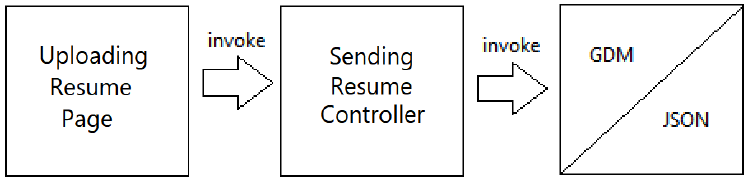
\includegraphics[width=13cm, height=2.7cm]{./images/7-6-1}
					\end{minipage}
				\end{flushleft}
			\end{minipage}
			
			\\
			\hline
			رفتاری & 
			\begin{minipage}{\textwidth}
				\begin{flushleft}
					\begin{minipage}{\textwidth}
						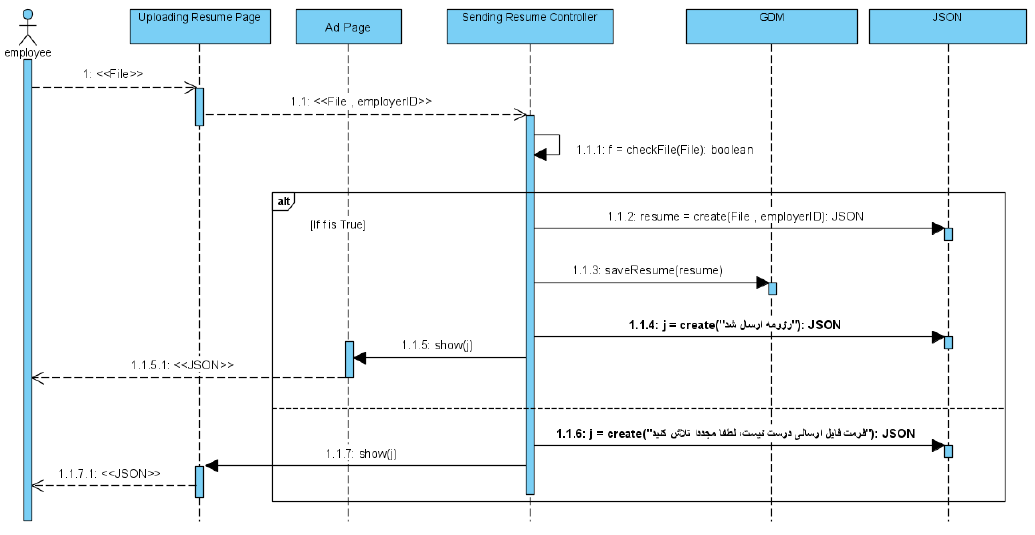
\includegraphics[width=13.5cm, height=6cm]{./images/7-6-2}
					\end{minipage}
				\end{flushleft}
			\end{minipage}
			\\
			\hline
		\end{tabular}
	\end{adjustbox}
	\caption{جدول \arabic{table}}
	\label{table-with-pic:6}
\end{table}

\begin{table}[H]
	\begin{adjustbox}{width=\textwidth}
		\begin{tabular}{|c|p{\textwidth}|}
			\hline
			نام &
			کنترل‌گر ثبت‌نام \\ 
			\hline
			گونه & 
			\grasp \\
			\hline
			خانواده &
			\controller \\
			\hline
			مسئله & 
			چه کسی مسئول رسیدگی به درخواست ثبت‌نام کاربر است؟\\
			\hline
			راه‌حل& 
			صفحه‌ی ثبت‌نام، اطلاعات را به کنترل‌گر ثبت‌‌نام می‌فرستد و نتبجه‌ را از کنترل‌گر دریافت می‌کند. \\
			\hline
			ساختاری & 
			\begin{minipage}{\textwidth}
				\begin{flushleft}
					\begin{minipage}{\textwidth}
						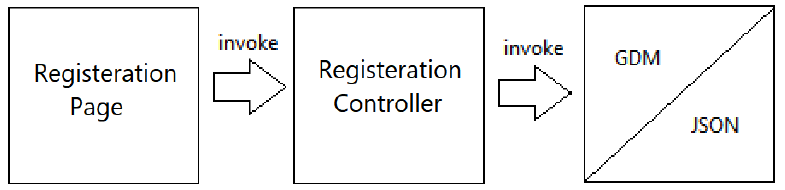
\includegraphics[width=13cm, height=2.7cm]{./images/7-7-1}
					\end{minipage}
				\end{flushleft}
			\end{minipage}
			
			\\
			\hline
			رفتاری & 
			\begin{minipage}{\textwidth}
				\begin{flushleft}
					\begin{minipage}{\textwidth}
						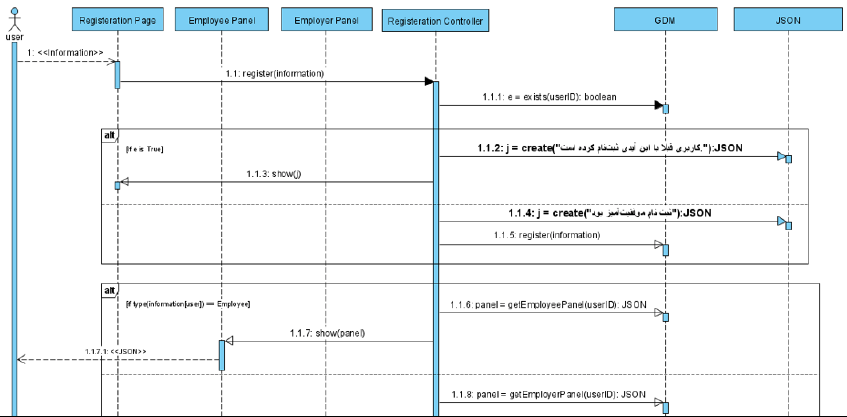
\includegraphics[width=13.5cm, height=6cm]{./images/7-7-2}
					\end{minipage}
				\end{flushleft}
			\end{minipage}
			\\
			\hline
		\end{tabular}
	\end{adjustbox}
	\caption{جدول \arabic{table}}
	\label{table-with-pic:7}
\end{table}
